% Created 2020-10-21 Wed 22:24
% Intended LaTeX compiler: pdflatex
\documentclass[11pt]{article}
\usepackage[utf8]{inputenc}
\usepackage[T1]{fontenc}
\usepackage{graphicx}
\usepackage{grffile}
\usepackage{longtable}
\usepackage{wrapfig}
\usepackage{rotating}
\usepackage[normalem]{ulem}
\usepackage{amsmath}
\usepackage{textcomp}
\usepackage{amssymb}
\usepackage{capt-of}
\usepackage{hyperref}
\usepackage{minted}
\author{Alex Elias}
\date{\today}
\title{}
\hypersetup{
 pdfauthor={Alex Elias},
 pdftitle={},
 pdfkeywords={},
 pdfsubject={},
 pdfcreator={Emacs 27.0.91 (Org mode 9.3.7)}, 
 pdflang={English}}
\begin{document}

\tableofcontents

Alex Elias 500407020

\section{Introduction}
\label{sec:orgbc75115}

Image data is an extremely abundant source of information in the modern world. It is also difficult to process and extract encoded information. Methods for information extraction from image data could hold a variety of use cases from robotics to security to home automation. Since image data is much higher dimension then traditional datasets, efficient methods for dimensionality reduction and prediction are necessary to achieve the best performance with as little cost in terms of hardware as necessary.

The specific problem of classification of fashion images is important as well, for example manual data entry of clothing is time consuming and error prone, and labels for products are not always accurate which may result in a loss of sales or customer frustration with online fashion resalers.

In this report, I will address a few methods for classification of image data, along with a few strategies for handling the high dimensionality of the data as well as selecting hyperparameters of chosen models for the specific problem of classification of fashion images.

Dimensionality Reduction methods include:
\begin{itemize}
\item Principle Component Analysis (PCA)
\item Non-Negative Matrix Factorization (NMF) (extra)
\end{itemize}

Prediction algorithms include:
\begin{itemize}
\item K-Nearest Neighbours (KNN)
\item Gaussian Naive Bayes (GNB)
\end{itemize}

With the problem that is being adressed here, there are 35000 images of a few categories of clothing items: 'T-shirt/top','Trouser', 'Pullover', 'Dress', 'Coat', 'Sandal', 'Shirt', 'Sneaker', 'Bag' and 'Ankle boot'. The images are paired with numbers 0 - 9 (in the order above). Of the 35000 images, all analysis was performed on 32,000 training examples. (often split into traning and validation sets of size 30,000 and 2,000 respectively)

\subsection{Language}
\label{sec:org6d05148}
In this report, I will refer to pixels of an image as 'features' and images as 'observations'. A single observation \(\mathbf{x}\) has \(m\) features. The \(i^{th}\) feature of \(x\) is denoted \(x_i\). In addition, the list of classes will be referred to by \(C\) and the \(i^{th}\) class is \(C_i\). a true label is denoted \(y\) and is a member of \(C\). \(\widehat y\) refers to the prediction, such that if the prediction is correct \(\widehat y = y\)

\section{Methods}
\label{sec:orgc47525f}
There were a few methods that were tested in this report.
\subsection{Gaussian Naive Bayes (GNB)}
\label{sec:orgad6d765}
This is a prediction model that uses bayesian statistics to predict a class label. It is defined by just a few formulae.

Generally, it makes the assumption that features are independant from each other. IE if one feature has a large/small value it has no effect on weather any other feature has a large/small value. (there is no correlation or interaction)

This allows for the data to be predicted by a product of conditional probabilities:

\begin{equation}
p\left(C_k\middle|\mathbf{x}\right) \propto p\left(C_k\right) \prod\limits_{i=1}^mp\left(x_i \middle|C_k\right)
\end{equation}


We can then select the most probable outcome:

\begin{equation}
\widehat {y} = \mbox{argmax}_{c \in C} \,p\left(c\middle|\mathbf{x}\right)
\end{equation}

Since we are selecting the argmax of the probabilities, we only need the order so proportional is good enough.

We estimate a normal distribution for \(p\left(x_i\middle|C_k\right)\) computing a mean and standard deviation over that class for that feature, allowing us to use the normal PDF to estimate probability for this property.

We estimate \(p\left(C_k\right)\) with:
  \begin{equation}
p\left(C_k\right) = {1\over n}\sum\limits_{i=0}^n \left\{\begin{array}{ll} 1 &: Y_i = C_k\\ 0 &: Y_i \ne C_k\end{array}\right|
  \end{equation}

\subsection{K-Nearest Neighbours (KNN)}
\label{sec:org26f623a}
This method estimates \(\widehat y\) by taking 'votes' from \(k\) nearest neighbours to \(\mathbf x\) in the data. This is done by computing the distance from \(\mathbf x\) to every observation in the training set, and selecting the \(k\) closest ones. Once these neighbours are known, they each vote their label to be the label that is predicted. In this implementation I have used weighted voting, meaning that the elements of the training set that are closer to \(\mathbf{x}\). I have weighted them by the inverse of the distance.
\subsection{NonNegative Matrix Factorization (NMF) (extra)}
\label{sec:org59e4451}
This creates a 'dictionary' of non-negative factors of the original dataset. These factors are then scaled by an also positive representation vector to sum to the original image. It did not work very well on this dataset. The hope is that it is more explainable then PCA while providing the benefits.

After the method is completed, it can easily transform an observation with \(m\) features and reduce it to a much smaller number, without losing much information.

\subsection{Principle Component Analysis (PCA)}
\label{sec:orgf4406f3}
Similar to NMF, PCA takes observations and represents them with smaller representation vectors.

This works by finding the direction (in \(m\) dimensions) in which there is the most variance, and projecting the data to have 0 variance along the perpendicular hyperplane. This direction becomes the first principle component. The process is repeated for \(k-1\) more principle components. (Numerically it works a little differently, but this is the intuition)

\section{Experimentation and Results}
\label{sec:orgda0f67e}

\subsection{Simple GNB}
\label{sec:org37e2ba9}

First, let us consider the computationally easiest model; GNB with no pre-processing. Here is a confusion matrix:
\begin{center}
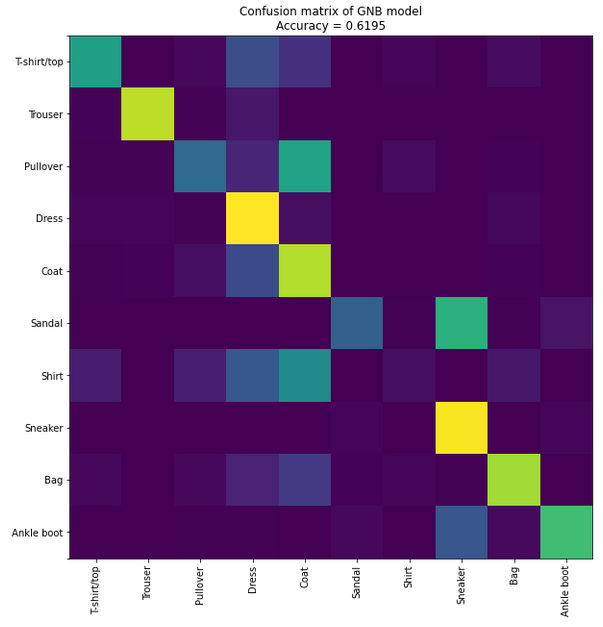
\includegraphics[width=.9\linewidth]{.images/Experimentation_and_Results/2020-10-21_19-58-52_screenshot.png}
\end{center}
the GNB model is extremely quick to fit and predict, as fitting a model requires computing mean and standard deviation of each feature (takes \(O\left(m|C|\right)\) time). Fitting is a quick product over all features, also taking very little time (also \(O\left(m |C|\right)\) time). I did not write any loops in python for this (utilizing the powerful numpy library) making my implementation extremely fast.

This shows that even the basic GNB model performs much better then random (accuracy of .1). But we can improve.

\subsection{Simple KNN}
\label{sec:org6b9b902}

Here is a KNN model (k=3)

\begin{center}
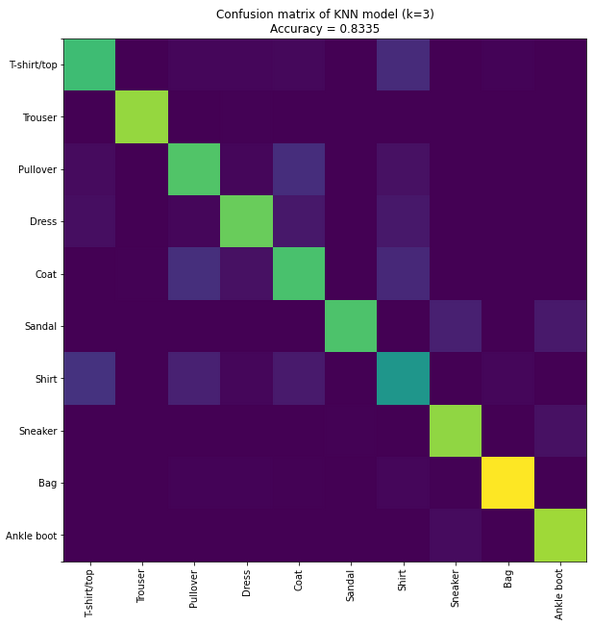
\includegraphics[width=.9\linewidth]{.images/Experimentation_and_Results/2020-10-21_20-06-57_screenshot.png}
\end{center}

Running a KNN model takes a much longer time (especially in my implementation) as the distance between a single observation \(\mathbf x\) and every observation in the training set must be computed (to find the k smallest distances). This results in a training time of 0 (as it just needs to save the training dataset) and a testing time of approximately \(O\left(nm\right)\) time (if computation of the distance takes \(m\) time). This is a problem as both \(n\) and \(m\) are very large numbers, making predicting many observations take even longer. The accuracy is much better then GNB however. In my implementation, again I have used very few python loops minimizing the language overhead.

\subsection{Dimensionality reduction with PCA}
\label{sec:orgfa782f9}

Dimensionality reduction techniques have multiple advantages. For the Gaussian Naive Bayes model, it indroduces some interaction between features (by making features functions of the reduced features) allowing some circumvention of the independance assumption. For the KNN model, it reduces the size of \(m\) that the KNN sees, thus reducing the overall runtime of the algorithm.

Since PCA works with minimizing variance along all axis, it is commonplace to normalize all features before performing the dimensionality reduction. Here is the PCA with a cutoff explaining 95\% of variation to the data on normalised data:
\begin{center}
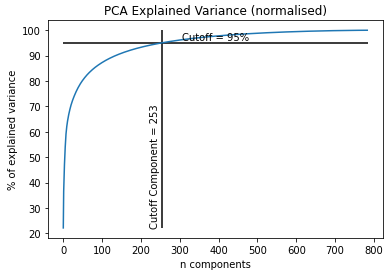
\includegraphics[width=.9\linewidth]{.images/Experimentation_and_Results/2020-10-21_20-25-19_screenshot.png}
\end{center}

In this dataset, the range of values is known, and there are many features (upon inspecting the dataset) that are never significant to the classification:

\begin{center}
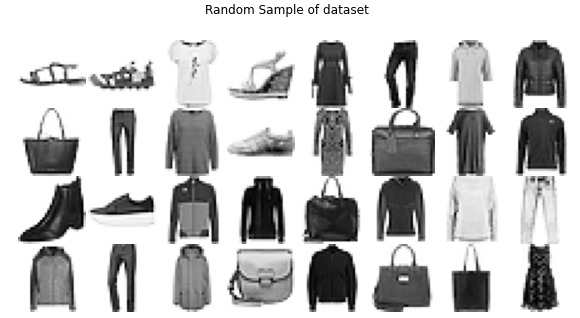
\includegraphics[width=.9\linewidth]{.images/Experimentation_and_Results/2020-10-21_20-29-28_screenshot.png}
\end{center}

(see all pixels in corner are always white)

With normalisation, these features always contribute the same amount to the variance. For this reason, I tried without normalisation:

\begin{center}
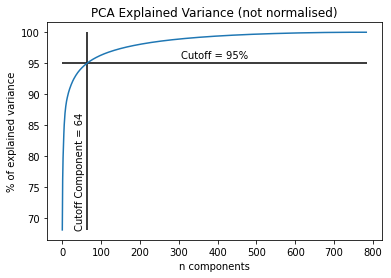
\includegraphics[width=.9\linewidth]{.images/Experimentation_and_Results/2020-10-21_20-31-11_screenshot.png}
\end{center}

There are far fewer components needed to explain 95\% of the variance (possibly because the PCA is not trying to explain all the noise in the corners equally to the pixel differences in the middle)

This is clear if you look at the components themselves: (taken by transforming one-hot vectors)

\begin{center}
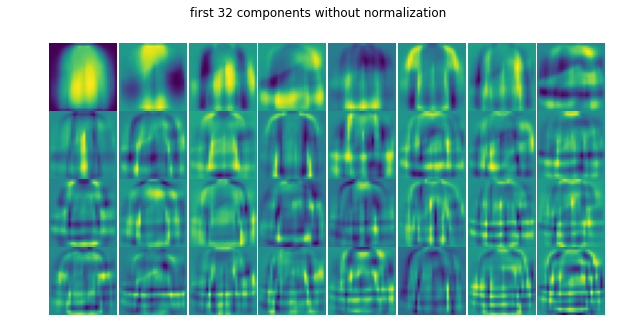
\includegraphics[width=.9\linewidth]{.images/Experimentation_and_Results/2020-10-21_20-35-29_screenshot.png}
\end{center}

\begin{center}
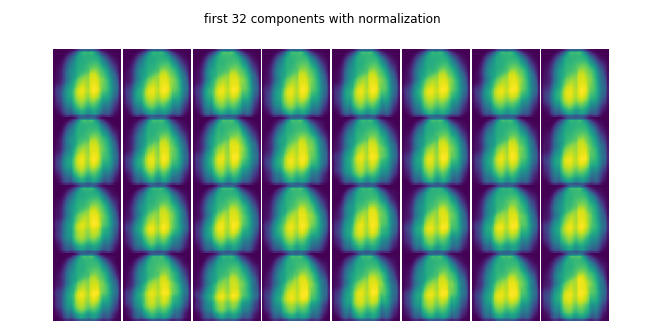
\includegraphics[width=.9\linewidth]{.images/Experimentation_and_Results/2020-10-21_20-35-49_screenshot.png}
\end{center}

\begin{center}
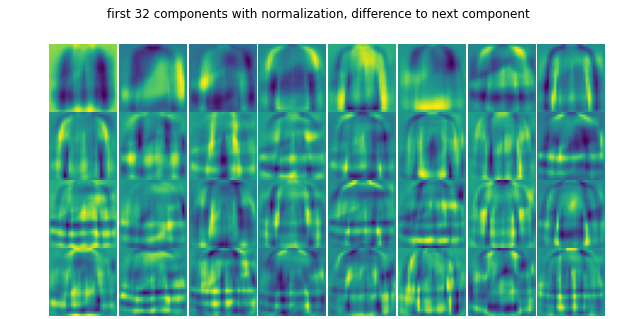
\includegraphics[width=.9\linewidth]{.images/Experimentation_and_Results/2020-10-21_20-36-09_screenshot.png}
\end{center}

\subsection{GNB with PCA}
\label{sec:org0034792}
As previously stated, GNB benefits from PCA as PCA introduces some interaction between features. Below is a plot demonstrating the relationship between GNB's accuracy and the number of components that the PCA uses:
\begin{center}
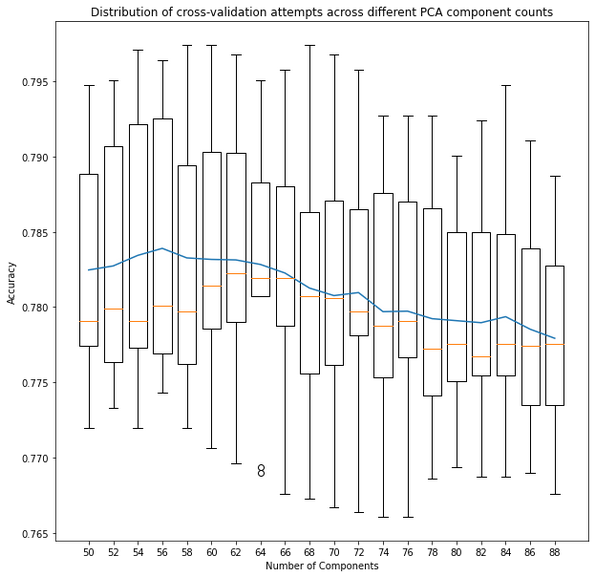
\includegraphics[width=.9\linewidth]{.images/Experimentation_and_Results/2020-10-21_20-39-46_screenshot.png}
\end{center}
the mean is the line in blue and medians are the orange bars in the boxplots.

This was generated using 10 fold cross validation on the entire 32,000 observation test+training set. (not the 3,000 reserved validation set)

Depending on the metric you are using (mean or median) the best number of components seems to be between 54 and 64, aligning with the results from the previous section. (as higher components are not representing meaningful data, meaning the GNB gets 'distracted' by them)

\subsection{Dimensionality reduction with NMF and GNB}
\label{sec:org3b2030f}
The aim of NMF is not the same as the aim of PCA, as it is attempting to produce a positive matrix representation while reducing the error. I thought this may further improve the performance of GNB as it may introduce even more relevant interaction between features. This was not the case however:
\begin{center}
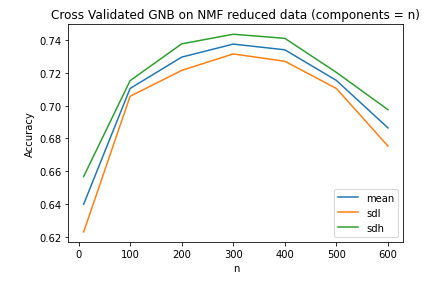
\includegraphics[width=.9\linewidth]{.images/Experimentation_and_Results/2020-10-21_21-07-43_screenshot.png}
\end{center}

sdl and sdh represent 1 standard deviation above and below the mean. The best performance of the GNB model here didnt quite make a mean accuracy of 0.74, but the minimum with PCA was about .78. This was a let down for me after so much time implementing.

\subsection{KNN with PCA}
\label{sec:org0fe5fa6}

Here was a quick grid search demonstrating the optimal k value for KNN:
\begin{center}
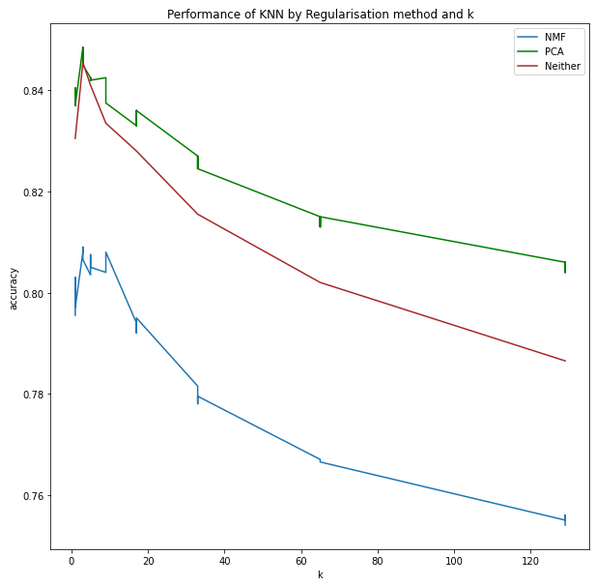
\includegraphics[width=.9\linewidth]{.images/Experimentation_and_Results/2020-10-21_21-17-50_screenshot.png}
\end{center}

This demonstrates 2 things:
\begin{enumerate}
\item the optimal number for k is approximately 6
\item at the optimal k, PCA and no reduction perform approximately equivalently, (and outside the optimal range PCA performs better then no reduction)
\end{enumerate}

It is also worth mentioning that I tried 3 different distance functions:
\begin{enumerate}
\item Cosine distance
\item Manhatten distance
\item euclidian distance
\end{enumerate}

Of these, manhatten distance performed the best. The following was the final tuning for finding the best parameter for pca components.

Here is the performance of the best model:

\begin{center}
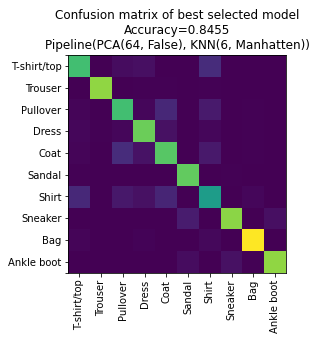
\includegraphics[width=.9\linewidth]{.images/Experimentation_and_Results/2020-10-21_22-15-36_screenshot.png}
\end{center}


\section{Conclusion}
\label{sec:org7239f13}

In this study, I determined the effectiveness of KNN, GNB, PCA and NMF on this fashion dataset. In the future, I would like to experiment with other models such as SVM and Multinomial Logistic Regression. I would also like to experiment more with NMF as it performed much worse then expected. Perhaps it would benefit from other loss functions?

PCA performed especially well on this dataset, reducing the dimensionality by about 90\%. This allowed KNN to run in reasonable time. The GNB model did surprisingly well given its independance assumption (even with PCA to re-introduce it) but it could not out-perform KNN.

The final best model was:
PCA(64, no-normalization) -> KNN(6, manhatten)

\section{Appendix}
\label{sec:org897e736}
The following libraries are required to run my notebook to predict:

The computer this was running on has an 10th generation i5-9300H @ 2.40GHz

\begin{itemize}
\item numpy 1.19.0
\item h5py 2.10.0
\item seaborn 0.11.0
\item matplotlib 3.2.2
\item (python 3.8.5 standard library)
\end{itemize}
\end{document}